

\chapter{Processos Estocásticos}

Até o momento, nossa análise considerou variáveis aleatórias independentes, uma
simplificação que facilitou a compreensão de conceitos fundamentais como
entropia e informação mútua. Ao final, chegamos à conclusão de que $nH(X)$ bits são
suficientes, na média, para representar uma sequência de $n$ variáveis aleatórias
independentes e identicamente distribuídas. Neste capítulo, removemos essa restrição para
abordar processos estocásticos, nos quais as variáveis aleatórias exibem
dependências temporais ou estruturais. Introduziremos a entropia de um processo
estocástico, que quantifica a incerteza associada a uma sequência de eventos, e
a taxa de entropia, uma medida assintótica da informação gerada por unidade de
tempo. Esses conceitos são essenciais para modelar sistemas dinâmicos. Em
particular, focaremos nas cadeias de Markov, um caso especial de processos
estocásticos em que a dependência é limitada ao estado imediatamente anterior,
oferecendo um equilíbrio entre simplicidade e aplicabilidade em problemas de
codificação e comunicação.

Um processo estocástico estacionário em sentido estrito é uma sequência de
variáveis aleatórias cujas propriedades estatísticas conjuntas permanecem
invariantes sob deslocamentos temporais. Isto implica que, por exemplo, médias,
variâncias e outras estatísticas não dependem do instante absoluto, permanecem
estáveis ao longo do tempo.

\begin{definition}[Processo Estocástico Estacionário (sentido-estrito)]
  Uma sequência de v.a.s. $X_1, X_2, \ldots, X_n$ é governada por uma distribuição probabilística é dita
  estacionária em sentido estrito se
  \begin{equation}
  p(X_{1:n} = x_{1:n}) = p(X_{1+l:n+l} = x_{1:n}) ,
  \end{equation}
  para todo $l$, todo $n$ e todo $x_{1:n} \in \mathcal{X}^n$.
\end{definition}

Um processo de Markov é um processo estocástico em que a probabilidade do
próximo estado depende apenas do estado atual, e não de toda a história
anterior.

\begin{definition}[Processo de Markov de primeira ordem]
  Um processo estocástico é um processo de Markov de primeira ordem se
  \begin{equation}
     p(X_{n+1} = x_{n+1} \mid X_{1:n} = x_{1:n}) = p(X_{n+1} = x_{n+1} \mid X_n = x_n)
  \end{equation}
\end{definition}
A essência de um processo de Markov reside na ideia de que, dado o estado
presente, o futuro e o passado são independentes. Em termos probabilísticos,
para o caso de primeira ordem, isto significa que $p(x_{1:n}) = p(x_1)p(x_2 \mid x_1) \ldots p(x_n \mid x_{n-1})$.
Essa independência condicional reflete a `falta de memória' do processo,
onde conhecer o estado atual basta, não sendo necessário avaliar a influência do passado.

De forma geral, podemos estender a ideia anterior para processos de Markov
de ordens superiores.
\begin{definition}[Processo de Markov de ordem $m$]
  Um processo estocástico é um processo de Markov de ordem $m$ se
  \begin{equation}
    p(X_{n+1} = x_{n+1} \mid X_{1:n} = x_{1:n}) = p(X_{n+1} = x_{n+1} \mid X_n = x_n, X_{n-1} = x_{n-1}, \ldots , X_{n-m} = x_{n-m}) .
  \end{equation}
\end{definition}
Neste caso, isto significa que $p(x_{1:n}) = p(x_{m+1} \mid x_{m}, x_{m-1},
\ldots, p(x_1)) \ldots p(x_{n-1} \mid x_{n-2}, x_{n-3}, \ldots, x_{n-m-1})
p(x_n \mid x_{n-1}, x_{n-2}, \ldots, x_{n -m})$.


Uma cadeia de Markov homogênea é um processo de Markov em que as probabilidades
de transição entre estados não variam com o tempo.
\begin{definition}[Cadeia de Markov homogênea]
  Uma cadeia de Markov é invariante no tempo (também chamada de homogênea) se $p(x_{n+1} \mid x_n)$ não
  depender do tempo, i.e., se
  \begin{equation}
    p(X_{n+1} = b \mid X_{n} = a) = p(X_2 = b \mid X_1 = a) \quad \forall a,b,n .
  \end{equation}
\end{definition}
Neste caso, a cadeia de Markov pode ser descrita por uma matriz de transição fixa $P = [p_{ij}]_{ij}$
em que $p_{ij} = p(X_{n+1} = j \mid X_{n} = i)$. Podemos representar esta cadeia de Markov como um grafo
com setas entre estados cuja probabilidade de transição não é nula.
O fato de ser homogênea também facilita o estudo de propriedades assintóticas,
como a taxa de entropia, como veremos adiante.

\begin{example}[Cadeia de Markov homogênea de primeira ordem]
  Vamos considerar neste exemplo uma cadeia de Markov homogênea de primeira ordem
  com 4 estados. Esta cadeia pode ser ser representada pela sua matriz de transição:
  \begin{equation}
  P = \begin{bmatrix}
          0 & p(2 \mid 1) & 0 & p(4 \mid 1) \\
          0 & p(2 \mid 2) & p(3 \mid 2) & 0 \\
          0 & 0 & 0 & p(4 \mid 3) \\
          0 & 0 & 0 & p(4 \mid 4) \\
          \end{bmatrix} ,
 \end{equation}
 ou, alternativamente, pelo grafo ilustrado na \Cref{fig:markov-example}

\begin{marginfigure}%
  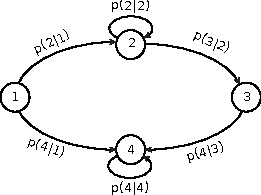
\includegraphics[width=\linewidth]{figures/markov-example.pdf}
  \caption{Exemplo de uma cadeia de Markov de primeira ordem com 4 estados.}
  \label{fig:markov-example}
\end{marginfigure}
\end{example}

Para uma cadeia de Markov homogênea de primeira ordem,
a probabilidade de um estado no instante $n+1$, pode ser dada em função dos possíveis
estados no instante $n$ e da probabilidade de transição:
\begin{equation}
  p(X_{n+1} = i) = \sum_{j} p(X_n = j) p(i|j) ,
\end{equation}
onde $p(i|j)$ é o elemento $p_{ij}$ da matriz de transição $P$. Esta cadeia de
Markov será estacionária se a probabilidade dos estados não mudar
ao longo do tempo, ou seja, $p(X_{n+1} = i) = p(X_n = i)$, para todo $i$.
Quando isto ocorrer, haverá uma distribuição estacionária $\mu$ tal que $\mu P = \mu$, onde $P$ é a matriz de transição.
Isto assegura que a probabilidade de cada estado permaneça constante ao longo do tempo quando o processo parte de,
ou alcança, uma distribuição $\mu$.

\begin{definition}[Cadeira de Markov irredutível]
  Uma cadeia de Markov é irredutível se $p_{ij}(n) > 0$ para todo $i,j$ e para algum $n$ onde
  $p_{ij}(n) = p(X_{n+1} = j \mid X_{n} = i)$.
\end{definition}
Ou seja, qualquer estado é acessível de qualquer outro estado (ao menos em algum instante $n$),
com probabilidade não nula.

\begin{definition}[Período de uma cadeia de Markov]
  Uma cadeia de Markov é periódica se $d(i) > 1$ com
  \begin{equation}
  d(i) = \gcd \{ n : p_{ii}(n) > 0 \}
  \end{equation}
  $d(i)$ é o período do $i$-ésimo estado.
\end{definition}
Note que temos o máximo divisor comum do número de épocas para o qual um retorno ao mesmo estado é possível.


\begin{example}[Cadeia de Markov homogênea de primeira ordem com dois estados]\label{ex:markovsimples2}
  Suponha uma cadeia de Markov homogênea de primeira ordem com apenas dois estados.
  Esta cadeia é caracterizada pela matriz de transição
  \begin{equation}
    P = \begin{pmatrix} 1 - \alpha & \alpha \\ \beta & 1 - \beta \end{pmatrix}
  \end{equation}
  e pode também ser representada pelo grafo da \Cref{fig:markov-example2}.
  \begin{marginfigure}%
  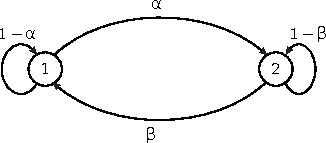
\includegraphics[width=\linewidth]{figures/markov-example2.pdf}
  \caption{Grafo representando uma cadeia de Markov de primeira ordem com dois estados.}
  \label{fig:markov-example2}
  \end{marginfigure}
  Se $\mu = [p_1 \ p_2]^T$ é uma distribuição estacionária, então devemos ter $\mu^T P = \mu^T$.
  Neste caso, teremos
  \begin{subequations}
  \begin{align}
    \mu^T = \begin{pmatrix} p_1 & p_2 \end{pmatrix} &= \begin{pmatrix} p_1 & p_2 \end{pmatrix} \begin{pmatrix} 1 - \alpha & \alpha \\ \beta & 1 - \beta \end{pmatrix} \\
          &= \begin{pmatrix} (1-\alpha) p_1 + \beta p_2 & \alpha p_1 + (1-\beta) p_2 \end{pmatrix}
  \end{align}
  \end{subequations}
  Obtemos assim:
  \begin{equation}
    p_1 = (1-\alpha) p_1 + \beta p_2
  \end{equation}
  logo, $p_1 = \frac{\beta}{\alpha} p_2$.
  Sabemos também que devemos ter $p_1 + p_2 = 1$. Por conseguinte, teremos
  \begin{subequations}
  \begin{align}
    p_1 + p_2 &= 1 \\
    \frac{\beta}{\alpha} p_2 + p_2 &= 1 \\
    p_2 &= \frac{\alpha}{\alpha + \beta} .
  \end{align}
  \end{subequations}
  Assim, teremos
  \begin{equation}
    \mu = \begin{pmatrix} \frac{\beta}{\alpha + \beta} \\ \frac{\alpha}{\alpha + \beta} \end{pmatrix} .
  \end{equation}
\end{example}



A Média de Cesàro representada uma técnica matemática que consiste em
substituir a soma parcial tradicional de uma série por uma média aritmética de
suas somas parciais.
Ela pode ser utilizada para obter representações mais precisas de sinais descontínuos;
reduzir artefatos processamento de sinais; aplicada a equações diferenciais parciais;
e, em processos estocásticos analisar o comportamento assintótico, especialmente ao 
estudar convergência ou taxas de entropia.

\begin{lemma}[Média Cesáro]
  Sejam $a_n$ números reais, se $a_n \rightarrow a$ quando $n \rightarrow \infty$ e $b_n = \frac{1}{n} \sum_{i=1}^n a_i$,
  então $b_n \rightarrow a$ quando $n \rightarrow \infty$.
\end{lemma}

\begin{proof}
  Como $a_n \xrightarrow[ n \rightarrow \infty ]{ } a$, para todo $\epsilon > 0$, existe $N_{\epsilon}$ tal que $\vert a_n - a \vert < \epsilon$
  para todo $n > N_{\epsilon}$.
  Para $n > N_{\epsilon}$ teremos
  \begin{subequations}
  \begin{align}
    \vert b_n - a \vert &= \vert \frac{1}{n} \sum_{i=1}^n a_i - a \vert = \vert \frac{1}{n} \sum_{i=1}^n a_i - \frac{1}{n} \sum_{i=1}^n a \vert \\
                        &= \vert \frac{1}{n} \sum_{i=1}^n (a_i - a) \vert  \leq  \frac{1}{n} \sum_{i=1}^n \vert a_i - a \vert \label{eq:demmediacesaro}\\
                        &= \frac{1}{n} \left( \sum_{i=1}^{N_{\epsilon}} \vert a_i - a \vert + \sum_{i=N_{\epsilon}+1}^n \vert a_i - a \vert \right) \\
                        &\leq \frac{1}{n} \sum_{i=1}^{N_{\epsilon}} \vert a_i - a \vert + \frac{1}{n}  \sum_{i=N_{\epsilon}+1}^n \epsilon \\
                &= \frac{1}{n} \sum_{i=1}^{N_{\epsilon}} \vert a_i - a \vert + \underbrace{\frac{n - N_{\epsilon}}{n}}_{<1} \epsilon \\
                &< \underbrace{ \frac{1}{n} \sum_{i=1}^{N_{\epsilon}} \vert a_i - a \vert }_{< \epsilon } + \epsilon < 2\epsilon \label{eq:demmediacesaro2}
  \end{align}
  \end{subequations}
  onde em \ref{eq:demmediacesaro} utilizamos a desigualdade triangular e em \ref{eq:demmediacesaro2}
  utilizamos o fato de que podemos tomar $n$ grande suficiente de forma que 
  $\frac{1}{n} \sum_{i=1}^{N_{\epsilon}} \vert a_i - a \vert < \epsilon$,
  pois trata-se de uma soma finita.

  Então $b_n \rightarrow a$ quando $n \rightarrow \infty$.
\end{proof}


Processos Estocástico possuem taxas de entropia, que intuitivamente representam o
quantidade de informação nova, na média, que é fornecida pelo processo estocástico a
cada instante.

\begin{definition}[Taxa de Entropia de um processo estocástico]
  A taxa de entropia de um processo estocástico $\{ X_i \}_i$ é definida como
  \begin{equation}\label{eq:txentropia}
    H(\mathcal{X}) \triangleq \lim_{n \rightarrow \infty} \frac{1}{n} H(X_1, X_2, \ldots, X_n) , 
    \end{equation}
quando existir.
\end{definition}

Observe que, na \Cref{eq:txentropia}, quando as v.a.s são i.i.d. teremos $H(X_1, \ldots, X_n) = H(X_1) + \ldots + H(X_n) = n H(X)$ e assim $H(\mathcal{X}) = H(X)$, ou seja,
\begin{equation}
  H(\mathcal{X}) = \lim_{n \rightarrow \infty} \frac{1}{n} H(X_{1:n}) = \lim_{n \rightarrow \infty} \frac{1}{n} \sum_{i=1}^n H(X_i) = H(X_1) .
\end{equation}
A taxa de entropia pode ser vista como a entropia por símbolo para um dado processo estocástico, quando $n$ cresce indefinidamente.



A Taxa de Entropia de um processo estocástico $H(\mathcal{X})$
mede a incerteza média por símbolo em uma sequência longa, 
enquanto a Taxa de Inovação da Informação $H'(\mathcal{X})$,
que será definida a seguir, quantifica a incerteza de um novo símbolo dado o passado. Para
processos gerais, essas taxas podem diferir devido à dependência entre
símbolos; no entanto, em processos estacionários, ambas
convergem ao mesmo valor, ou seja, $H(\mathcal{X}) = H'(\mathcal{X})$,
refletindo a estabilidade estatística do processo ao longo do tempo.

 \begin{definition}[Taxa de Inovação da Informação]
  Vamos assumir um processo estocástico e definir a taxa da seguinte forma
  \begin{equation}
    H'(\mathcal{X}) \triangleq \lim_{n \rightarrow \infty} H(X_n \mid X_{n-1}, X_{n-2}, \ldots , X_1) ,
  \end{equation}
  se existir.
 \end{definition}
 Veremos a seguir que $H'(\mathcal{X})$ existe para um processo estocástico estacionário.

 \begin{theorem}[Um processo estocástico estacionário possui taxa de inovação de informação]
  Para um processo estocástico estacionário, $H(X_n \mid X_{n-1}, X_{n-2}, \ldots , X_1)$ é decrescente com $n$ e possui como limite $H'(\mathcal{X})$.
\end{theorem}
\begin{proof}
  \begin{subequations}
  \begin{align}
  H(X_{n+1} \mid X_1, \ldots, X_n) &\leq H(X_{n+1} \mid X_2, \ldots, X_n) \\
                &= H(X_n | X_1, \ldots, X_{n-1})
  \end{align}
  \end{subequations}
  Onde utilizamos o fato de que condicionar não aumenta (decresce ou não altera) a entropia;
  e utilizamos o fato de que o processo estocástico é estacionário.

  Temos então uma sequência decrescente com limite inferior $0$, logo, esta sequência possui um limite: $H'(\mathcal{X})$.
\end{proof}

\begin{theorem}[Em um processo estocástico estacionário taxa de inovação é igual a taxa de entropia]
  Para um processo estocástico estacionário temos
  \begin{subequations}
  \begin{align}
    \lim_{n \rightarrow \infty} H(X_n \mid X_{n-1}, X_{n-2}, \ldots, X_1) &\triangleq H'(\mathcal{X}) \\
                                                                          &= H(\mathcal{X}) \triangleq \lim_{n \rightarrow \infty} \frac{1}{n} H(X_1,X_2,\ldots,X_n)
  \end{align}
  \end{subequations}
\end{theorem}

\begin{proof}
  \begin{equation}
        b_n = \frac{H(X_1,X_2,\ldots,X_n)}{n} = \frac{1}{n} \sum_{i=1}^n \underbrace{H(X_i \mid X_{i-1}, \ldots, X_1)}_{=a_i} ,
  \end{equation}
  como $a_n \rightarrow H'(\mathcal{X})$, teremos $b_n \rightarrow H'(\mathcal{X})$, mas por definição $b_n \rightarrow H(\mathcal{X})$.
\end{proof}



\begin{example}[Taxa de entropia para cadeia de Markov de primeira ordem]
  A taxa de entropia para um cadeia de Markov de primeira ordem estacionária será dada da seguinte forma
  \begin{subequations}\label{eq:extxentropiamarkov1ord}
  \begin{align}
  H(\mathcal{X}) &= H'(\mathcal{X}) = \lim_{n \rightarrow \infty} H(X_n \mid X_{n-1}, \ldots, X_1) \\
        &= \lim_{n \rightarrow \infty} H(X_n \mid X_{n-1}) \\
        &= H(X_2 \mid X_1) \label{eq:extxentropiamarkov1ordd}\\
        &= - \sum_{x_2, x_1} p(x_2, x_1) \log p(x_2 \mid x_1) \\
        &= \sum_i \mu_i \left[ - \sum_j p_{ij} \log p_{ij} \right] ,
  \end{align}
  \end{subequations}
  onde $\mu$ é a distribuição estacionária, $p_{ij}$ a probabilidade de transição de $i$ para $j$ e,
  em \ref{eq:extxentropiamarkov1ordd}, utilizamos o fato de termos uma cadeia de Marvov de primeira ordem estacionária.
\end{example}

\begin{example}[Markov com apenas dois estados]
  Para a cadeia de Markov simples apresentada no \Cref{ex:markovsimples2}, teremos
  \begin{equation}
    H(\mathcal{X}) = H(X_2 \mid X_1) = \frac{\beta}{\alpha + \beta} H(\alpha) + \frac{\alpha}{\alpha + \beta} H(\beta) .
  \end{equation}
\end{example}


\begin{example}[Modelos de Ehrenfest]
Os Modelos de Ehrenfest são cadeias de Markov que descrevem a dinâmica de
partículas em um sistema com dois compartimentos. Tais modelos são
frequentemente usados para ilustrar conceitos de equilíbrio estatístico e
comportamento assintótico. A análise desse processo estocástico revela
propriedades como estacionaridade e convergência para uma distribuição de
equilíbrio. Paul Ehrenfest propôs um modelo simples para a troca de calor ou
moléculas entre dois corpos isolados. Neste modelo da cadeia de Ehrenfest
iremos considerar a troca de moléculas de gás entre dois compartimentos,
rotulados por 0 e 1, conforme apresentado na \Cref{fig:ehrenfest}.
\begin{marginfigure}%
  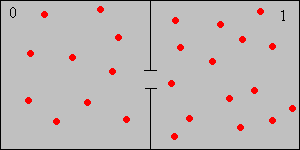
\includegraphics[width=\linewidth]{figures/ehrenfest.png}
  \caption{Exemplo de uma cadeia de Markov de primeira ordem com 4 estados.}
  \label{fig:ehrenfest}
\end{marginfigure}
Partículas movem-se aleatoriamente entre os
compartimentos com probabilidades fixas, e o estado do sistema é representado
pelo número de partículas em um dos compartimentos.
Iremos denotar por $X_k$ o número de partículas no compartimento 1 no instante $k$.
$X_k$ descreve o estado atual do sistema. Temos um processo estocástico gerando $X_{1:n}$,
onde $X_k \in \{0,1,\ldots,m\}$.

Supondo que no instante $k$ o compartimento 1 possua $i$ partículas ($X_k = i$).
O modelo de Ehrenfest nos fornece:
\begin{subequations}
\begin{align}
\Pr(X_{k+1} = i+1 | X_k = i) &= \frac{m - i}{m} , \\
\Pr(X_{k+1} = i-1 | X_k = i) &= \frac{i}{m} .
\end{align}
\end{subequations}

Neste modelo a propriedade de Markov é satisfeita:
\begin{subequations}
\begin{align}
\Pr(X_{n+1} = i+1 | X_0 = i_0, X_1 = i_1, \ldots, X_{n-1} = i_{n-1}, X_n = i) &=& \Pr(X_{n+1} = i+1 | X_n = i) , \\
\Pr(X_{n+1} = i-1 | X_0 = i_0, X_1 = i_1, \ldots, X_{n-1} = i_{n-1}, X_n = i) &=& \Pr(X_{n+1} = i-1 | X_n = i) . 
\end{align}
\end{subequations}
A distribuição condicional não depende de $n$, desta forma, temos um processo estocástico homogêneo.
A cadeia de Markov poderá então ser descrita por uma matriz de transição fixa $P = [p_{ij}]_{ij}$.

Para $m = 4$ teremos a cadeia de Markov representada pelo grafo apresentado na \Cref{fig:ehrenfestm4}.
\begin{figure}%
\begin{tikzpicture}[->, >=stealth', auto, semithick, node distance=2.5cm]
\tikzstyle{every state}=[fill=white,draw=black,thick,text=black,scale=1]
\node[state]    (0)               {$0$};
\node[state]    (1)[right of=0]   {$1$};
\node[state]    (2)[right of=1]   {$2$};
\node[state]    (3)[right of=2]   {$3$};
\node[state]    (4)[right of=3]   {$4$};
\path
(0) edge[bend left,above]   node{$1$}    (1)
(1) edge[bend left,below]   node{$1/4$}  (0)
(1) edge[bend left,above]   node{$3/4$}  (2)
(2) edge[bend left,below]   node{$1/2$}  (1)
(2) edge[bend left,above]   node{$1/2$}  (3)
(3) edge[bend left,below]   node{$3/4$}  (2)
(3) edge[bend left,above]   node{$1/4$}  (4)
(4) edge[bend left,below]   node{$1$}    (3) ;
% edge[loop left]     node{$p^2$}         (1) ;
\end{tikzpicture}
  \caption{Modelo de Ehrenfest com 4 estados.}
  \label{fig:ehrenfestm4}
\end{figure}

Para este modelo, a matriz de transição é
\begin{equation}
\mathbf{P} =
\begin{blockarray}{cccccc}
0 & 1 & 2 & 3 & 4 \\
\begin{block}{(ccccc)c}
  0   & 1   & 0   & 0   & 0   & 0 \\
  1/4 & 0   & 3/4 & 0   & 0   & 1 \\
  0   & 1/2 & 0   & 1/2 & 0   & 2 \\
  0   & 0   & 3/4 & 0   & 1/4 & 3 \\
  0   & 0   & 0   & 1   & 0   & 4 \\
\end{block}
\end{blockarray}
\end{equation}

A distribuição de estado estacionário é tal que $\mathbf{\mu}^T P = \mathbf{\mu}^T$, com $\sum_i \mu_i = 1$.

\begin{subequations}
\begin{align}
\mathbf{\mu}^T P &= \mathbf{\mu}^T \\
\mathbf{\mu}^T (P-I) &= 0 \\
\mathbf{\mu}^T Q &= 0
\end{align}
\end{subequations}


Teremos aqui
\begin{equation}
Q = \begin{pmatrix}
-1  &  1  & 0   & 0   & 0   \\
1/4 & -1  & 3/4 & 0   & 0   \\
0   & 1/2 & -1  & 1/2 & 0   \\
0   & 0   & 3/4 & -1  & 1/4 \\
0   & 0   & 0   & 1   & -1
\end{pmatrix} .
\end{equation}

Vamos incorporar a condição $\sum_i \mu_i = 1$ fazendo:
\begin{equation}
\tilde{Q} = \begin{pmatrix}
-1  &  1  & 0   & 0   & 1 \\
1/4 & -1  & 3/4 & 0   & 1 \\
0   & 1/2 & -1  & 1/2 & 1 \\
0   & 0   & 3/4 & -1  & 1 \\
0   & 0   & 0   & 1   & 1
\end{pmatrix} ,
\end{equation}
e o novo sistema de equações será
\begin{equation}\label{eq-novo-sistema}
\mathbf{\mu}^T \tilde{Q} = (0, 0, 0, 1) .
\end{equation}

Para solucionar a Equação \ref{eq-novo-sistema}, iremos pós multiplicar ambos os lados
pela matriz inversa de $\tilde{Q}$,
\begin{equation}
\mathbf{\mu}^T = (0, 0, 0, 1) \tilde{Q}^{-1} ,
\end{equation}
obtendo assim
\begin{equation}
\mathbf{\mu}^T = \left( \frac{1}{16}, \frac{1}{4}, \frac{6}{16}, \frac{1}{4}, \frac{1}{16} \right)
\end{equation}

Conforme vimos na \Cref{eq:extxentropiamarkov1ord}, a taxa de entropia para um
cadeia de Markov de primeira ordem estacionária será dada da seguinte forma
\begin{equation}
  H(\mathcal{X}) = \sum_i \mu_i H( \mathbf{p_i} ) ,
\end{equation}
onde $\mu$ é a distribuição estacionária,
$p_{ij}$ a probabilidade de transição de $i$ para $j$ (elementos da matriz $P$)
e $\mathbf{p_i}$ a $i$-ésima linha da matriz $P$ (as probabilidades de transição à partir
do estado $i$).

Para o exemplo em questão:
\begin{subequations}
\begin{align}
  H(\mathcal{X}) &= \mu_1 H(\mathbf{p_1}) + \mu_2 H(\mathbf{p_2}) + \mu_3 H(\mathbf{p_3}) + \mu_4 H(\mathbf{p_4}) + \mu_5 H(\mathbf{p_5}) \\
        &= \frac{1}{16} H(0,1,0,0,0) + \frac{1}{4} H(\frac{1}{4}, 0, \frac{3}{4}, 0, 0) + \frac{6}{16} H(0, \frac{1}{2}, 0, \frac{1}{2}, 0) +
                \frac{1}{4} H(0, 0, \frac{3}{4}, 0, \frac{1}{4}) + \frac{1}{16} H(0, 0, 0, 1, 0) \\
        &= 0 + 2 \times \frac{1}{4} \left( \frac{1}{4} \log 4 + \frac{3}{4} \log \frac{4}{3} \right) +
                \frac{6}{16} + 0 \\
        &= \frac{1}{2} \left( \frac{1}{2} + \frac{3}{2} - \frac{3}{4} \log 3  \right) + \frac{6}{16} \\
        &= 1 - \frac{3}{8} \log 3 + \frac{6}{16} = \frac{11}{8} - \frac{3}{8} \log 3 = 0.78064
\end{align}
\end{subequations}

\end{example}
